\chapter{Microsoft Azure}
Jest to rozwiązanie chmurowe udostępnione przez firmę Microsoft.\ Zawiera wiele usług i narzędzi z zakresu zarządzania IT.\ W trakcie rejestracji na platformie nie jest pobierana opłata.\ Opłacie podlega jedynie wykorzystywanie konkretnych usług oraz zasobów platformy. \ Jest to model \textit{płatność za użycie} \textit{(ang: pay-per-use)}.
\\ \\
Początki platformy sięgają 2008 roku, kiedy do użytku został oddany Windows Azure.\ Narzędzie było zbudowane z modułów Windows NT.\ Windows Azure zawierał ograniczoną liczbę usług w chmurze.\ W kolejnych latach rozbudowano Windows Azure o relacyjne bazy danych SQL Azure oraz obsługę języków takich jak Java czy PHP.\ W 2010 oddano po raz pierwszy platformę do użytku komercyjnego.\ W tej wersji dodano między innymi:
\begin{itemize}
\item .NET Framework 4 związanego z Microsoft SQL Server,
\item obsługę aplikacji pisanych w wielu językach (takich jak C\#, Java, PHP)
\item sieć dostarczania zawartości \textit{(ang. Content Delivery Network, CDN)}.
\end{itemize}
Następnie wdrożono oprogramowanie typu open source oraz infrastrukturę definiowaną jako serwis \textit{(ang. Infrastructure-as-a-Service, IaaS)}.\ Zmieniono też nazwę na Microsoft Azure.\ W kolejnej generacji Microsoft zaadaptował rozwiązania Big Data do swojej platformy, umożliwiając korzystanie z języka \textit{R}, połączenie do Power BI, a także umożliwienie połączenia do rozwiązań end-to-end.
\\ \\
W czwartej generacji platformy, Microsoft skupił się na rozwiązaniach uczenia maszynowego oraz integracji z bazami danych, dzięki czemu powstało Azure Machine Learning Studio (Azure ML) oraz Azure Machine Learning Operations (MLOps).
\\ \\
Obecnie platforma została wzbogacona o Kubernetesa, dzięki czemu konteneryzacja ułatwiła pracę z klastrami wirtualnymi.\ Wirtualne klastry pozwalają na wydajniejszy i wygodniejszy sposób zarządzania aplikacjami i usługami.\ Dodatkowo zostało udostępnione wiele kombinacji usług technologicznych:

\begin{itemize}
    \item aplikacja jako usługa \textit{(ang. Software-as-a-Service, SaaS)},
    \item interfejs jako usługa \textit{(ang. Infrastucture-as-a-Service, IaaS)},
    \item platforma jako usługa \textit{(ang. Platfrom-as-a-Service, PaaS)}.
\end{itemize}
Dzięki powyższym usprawnieniom Microsoft dostarcza platformę przyjazną użytkownikowi, która umożliwia korzystanie z ponad 200 różnych usług opartych między innymi o rozwiązania chmurowe i sztuczną inteligencję~\cite{Roosevelt2022, MicrosoftAzurec, Datashift}.

\vfill
\pagebreak

\refsource{Rysunek}{fig:ms-azure} pokazuje obecny podział usług na platformie Microsoft Azure.\ Można wyróżnić wiele obszarów między innymi z zakresu bezpieczeństwa, zarządzania danymi, usług deweloperskich, analizy danych czy platformy aplikacji.

\begin{figure}[H]
    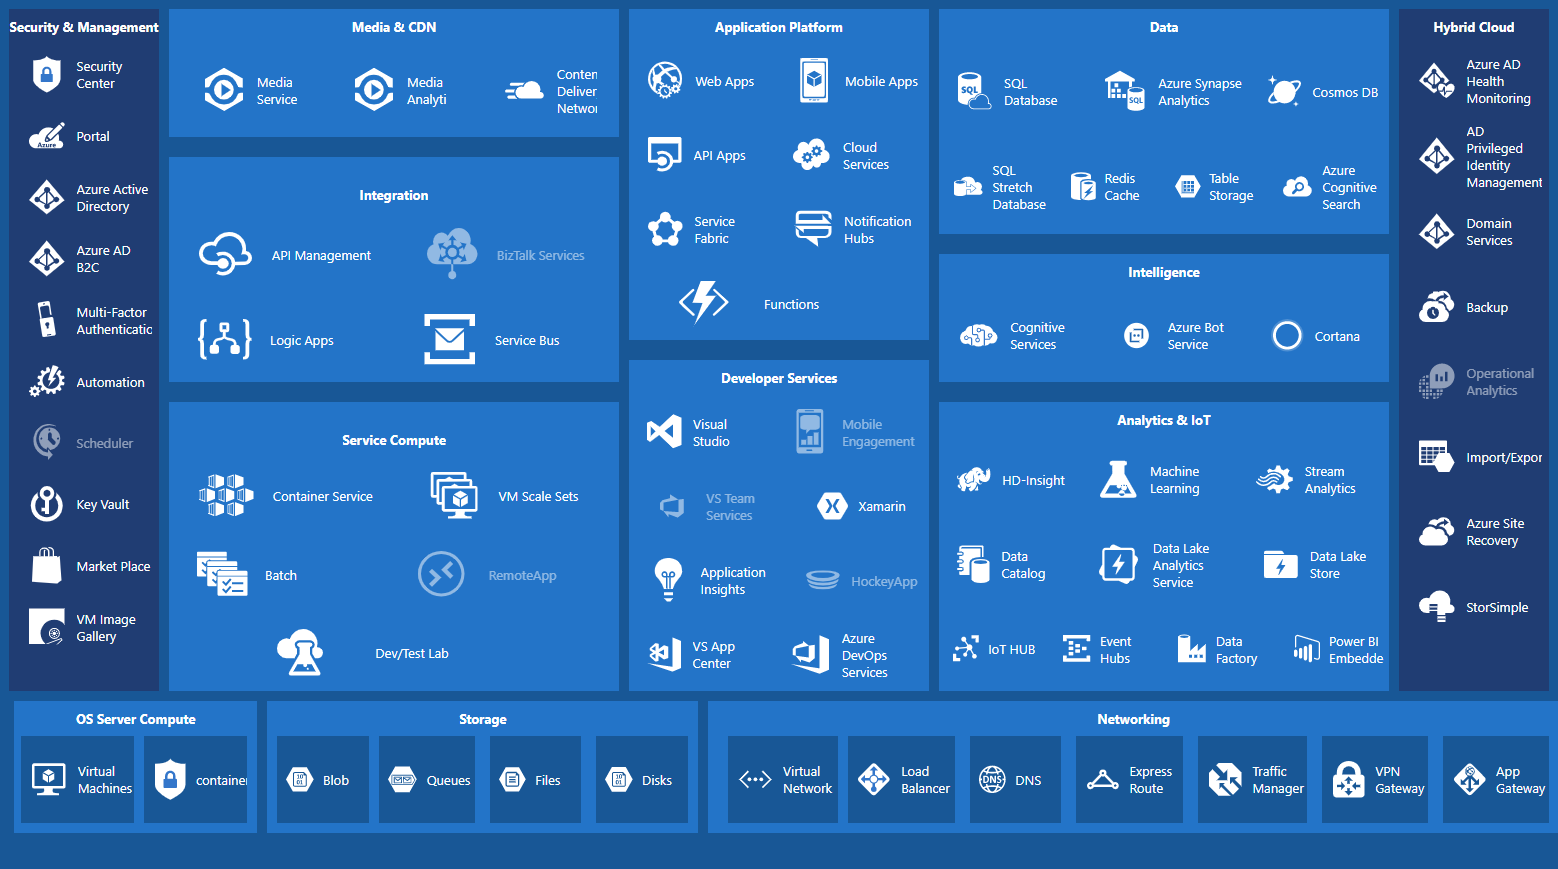
\includegraphics[width=\textwidth]{images/ms_azure}
    \captionsource{Schemat podziału usług MS Azure}{\cite{Datashifta}}
    \label{fig:ms-azure}
\end{figure}

\section{Infrastruktura}
Infrastruktura globalna Azure składa się z dwóch części: fizycznej infrastruktury oraz globalnej łączności.\ Infrastruktura fizyczna składa się z ponad 200 centrów danych rozmieszczonych na całym świecie, połączonych w jedną globalną sieć.\ Takie rozwiązanie umożliwia wysoką skalowalność i dostępność poszczególnych rozwiązań.\ Cały ruch sieciowy jest utrzymywany w prywatnej sieci Microsoft.\ Pozwala to na zachowanie informacji o adresach IP wewnątrz sieci, a co za tym idzie, informacje te nie trafiają do opinii publicznej~\cite{MicrosoftAzureb}.\\ \\

Na swojej stronie internetowej Microsoft udostępnia wirtualną mapę, umożliwiającą zobaczenie aktualnej sieci Microsoftu oraz jej rozmieszczenie na globie ziemskim.\ Podgląd przedstawiono na \refsource{rysunku}{fig:azure-ic}.
\vfill
\pagebreak

\begin{figure}[H]
    \begin{subfigure}[m]{0.7\textwidth}
    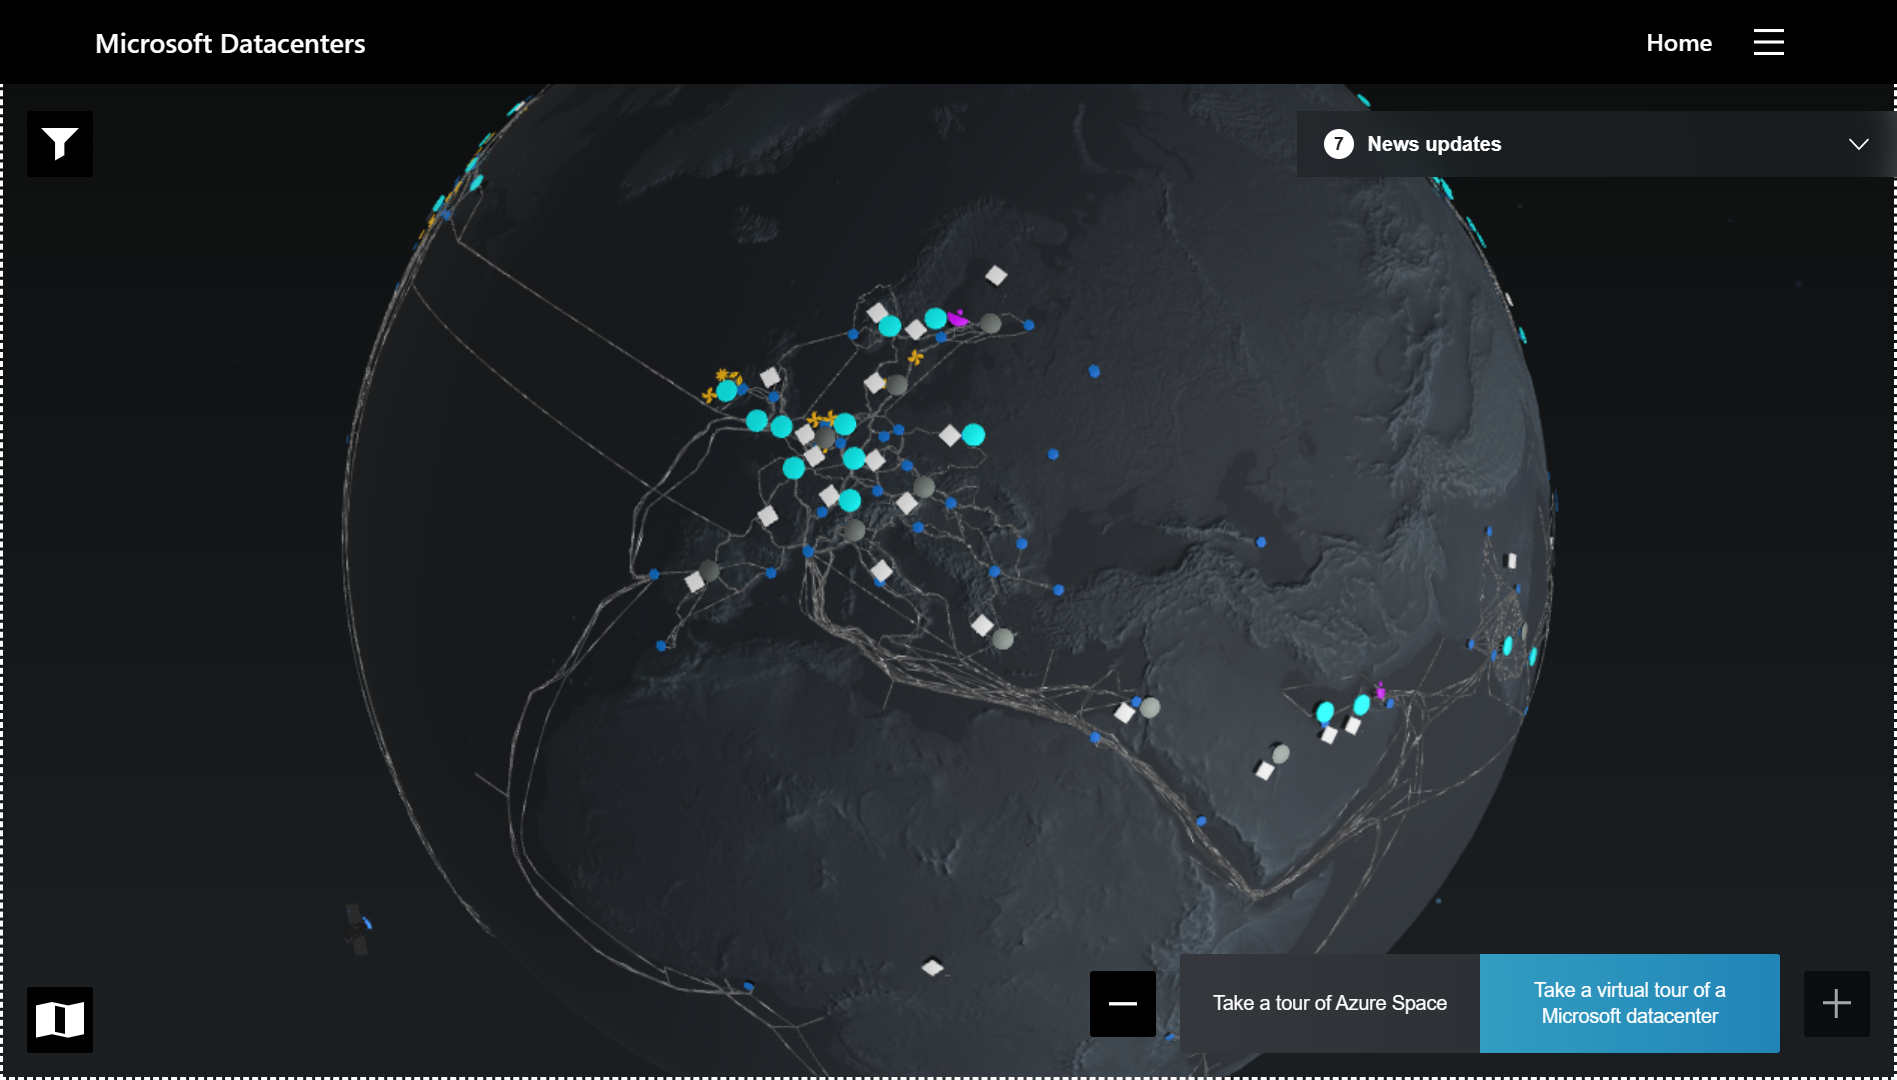
\includegraphics[width=\textwidth]{images/azure-ic}
    \caption{Globalna mapa infrastruktury sieciowe}
    \end{subfigure}
    \hfill
    \begin{subfigure}[m]{0.25\textwidth}
        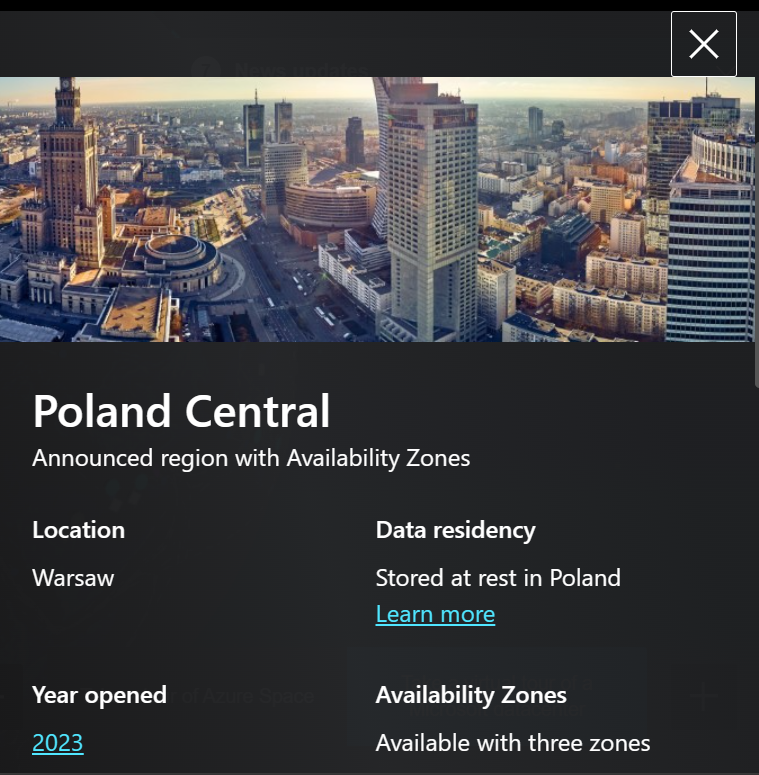
\includegraphics[width=\textwidth]{images/azure-pl}
        \caption{Informacje o centrum danych}
    \end{subfigure}
    \captionsource{Zdjęcia z mapy insfrastruktury Microsoft Azure}{\cite{MicrosoftAzuree, MicrosoftAzured}}
    \label{fig:azure-ic}
\end{figure}

Interaktywna mapa prezentuje informację o poszczególnych krajach oraz centrach danych znajdujących się na terytoriach tych krajów.

\section{Machine Learning Studio}
Azure Machine Learning (ML) to rozwiązanie dostarczane przez Microsoft Azure.\ Opiera się o ideę low-code/no-code, która została opisana w \refsource{rozdziale}{cha:low}.\ Usługa ML umożliwia łatwe i szybkie tworzenie wysoce wydajnych modeli uczenia maszynowego, a także zarządzanie nimi.\ Użytkownik nie musi posiadać wiedzy teoretycznej związanej z uczeniem maszynowym czy programowaniem.\ Rozwiązanie wspiera pełen cykl życia kompleksowego uczenia maszynowego.\ Taki cykl obejmuje natępujące etapy:
\begin{itemize}
    \item etykietowanie i przygotowywanie danych,
    \item budowanie i trenowanie modeli SI i ML,
    \item walidację i wdrażanie procesu uczenia się,
    \item zarządzanie i monitorowanie uzyskanych wyników~\cite{MicrosoftAzurel}.
\end{itemize}


Platforma umożliwia tworzenie potoków zadań, które połączone w jeden potok, wykonują poszczególne zadania w odpowiedniej kolejności.\ Mechanizm ,,\textit{złap i upuść}'' \textit{(ang. drag\&drop)} umożliwia tworzenie potoków w sposób graficzny.\ Dzięki modułowej budowie potoków można uzyskać rozwiązanie wielokrotnego użytku.\ W ramach jednego doświadczenia każdy moduł może byc buforowany.\ Pozwala to na ,,zapamiętanie'' wyniku poprzedniego uruchomienia i wykorzystanie go ponownie (o ile dane wejściowe albo konfiguracja nie uległy zmianie).\ Dodatkowo poza predefiniowanymi operacjami można wykorzystać moduły języka Python/R.\ Kolejną możliwością jest wytworzenie rozwiązania w technologii ,,\textbf{Jupiter Notebook}'' oraz wizualne narzędzie wykorzystujące mechanizm \textit{przeciągnij i upuść} \textit{(ang. Drag \& Drop)}.\ Rozwiązanie to pozwala układać ,,\textit{kafelki}'' służące do tworzenia potoków zadań.\ Każde zadanie wykorzystuje wcześniej przygotowaną jednostkę obliczeniową, dzięki czemu można przewidzieć albo dostosować koszt wykorzystania modelu.\ Umożliwione zostało również wdrażanie modeli jako punktów końcowych.\ Pozwala to na komunikowanie się z nimi za pomocą REST API.
\\ \\
Microsoft pobiera płatność jedynie za użytkowanie usług, co oznacza, że jeśli klaster komputerowy był wykorzystywany jedynie przez 1 godzinę, to za tą jedną godzinę zostanie obciążony klient \cite{MicrosoftAzuref}.